\section{Temporal Replication and Mining}
\label{sec:trm}
We resort to the MapReduce (MR) paradigm for designing 
a scalable parallel solution in mining GCMP. It is straightforward 
to partition the trajectory database into equal-sized 
temporal segments; and then mining the GCMP patterns out of each segments. However, GCMP
patterns may cross multiple temporal segments. To ensure
the correctness, we need to guarantee that
every valid pattern can be mined within at least 
one partitions.
Thus, some snapshots need to be 
replicated several times in multiple partitions. This
leads us to design the \emph{Temporal Replication and Mining}
(TRM) algorithm.

The work flow of TRM is illustrate as in Figure~\ref{fig:trm}. 
In brief, there are two pipeline MR jobs which further consist of four stages. 
The first MR job is considered as a preprocessing, where input trajectories
are grouped into snapshots and each snapshot runs a clustering method (e.g., Disk-based, DBSCAN, etc.).
The output is shown as in Figure~\ref{fig:trm}(b). The second
MR job is the \emph{TRM} algorithm. In the \emph{map} phase 
(i.e., Figure~\ref{fig:trm} (c)), temporally closed snapshots are grouped
into a partition. In the \emph{reduce} phase (i.e., Figure~\ref{fig:trm} (d)),
a \emph{Line Sweeping} method is developed to discover GCMP in each partition. Finally,
patterns from different partitions are then collected to form the output.

\begin{figure*} [t]
\center
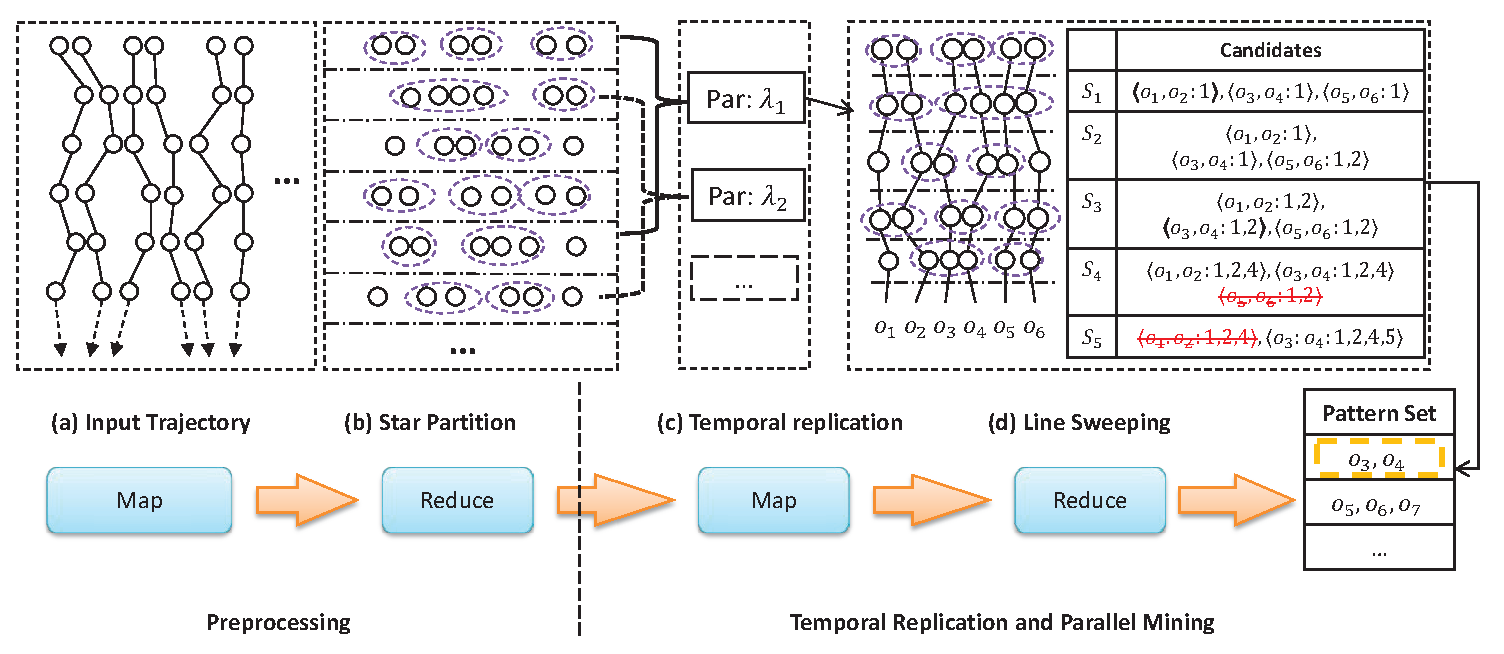
\includegraphics[width=\textwidth]{trm.eps}
\caption{Work flow of Temporal Replication and Mining. (a)(b) correspond to the first MR job which computes the clusters at each snapshot; 
(c)(d) correspond to the second MR job which uses TRM to mine GCMP in parallel.}
\label{fig:trm}
\end{figure*}

Since in the first MR job, each partition contains only one snapshot
for clustering, it is not necessary to replicate any snapshot. Thus, we
focus on describing the second MR job which is the \emph{Temporal
Replication and Mining} algorithm. We use $R$ to denote the replication factor.
The outline of TRM is 
shown in Algorithm~\ref{algo:trm_overview}.

\begin{algorithm}
\caption{Temporal Replication and Mining}
\label{algo:trm_overview}
\begin{algorithmic}[1]
\Require list of $\langle t, S_t \rangle$ pairs
\State $R \gets (\lceil \frac{K}{L} \rceil -1)*G+2K$
\State {---Map Phase---}
\label{code:trm-map-start}
\ForAll{$\langle t, S_t \rangle$}
	\ForAll{$i \in 1...R$}
		\State emit a $\langle t-i, S_t \rangle$ pair
	\EndFor  
\EndFor
\label{code:trm-map-end}
\State {---Partition and Shuffle Phase---}
\label{code:trm-par-start}
\ForAll{$\langle t, S \rangle$ pair} 
\State group-by $t$, emit a $\langle t, Par_t\rangle$
\State where $Par_t = \{S_t, S_{t+1}, .. S_{t+R}\} $
\EndFor
\label{code:trm-par-end}
\State {---Reduce Phase---}
\label{code:trm-red-start}
\ForAll{$\langle t,Par_t \rangle$}
\State lineSweepMining($Par_t$)
\label{code:trm-red-end}
\EndFor
\end{algorithmic}
\end{algorithm}

As shown in Algorithm~\ref{algo:trm_overview}, the TRM algorithm contains
three steps. First, in the map phase, each snapshot is keyed 
with its timestamp (lines~\ref{code:trm-map-start}-\ref{code:trm-map-end}). 
Second, in the partition phase, every snapshot is grouped with its next 
$R$ snapshots to form a partition (lines~\ref{code:trm-par-start}-\ref{code:trm-par-end}). 
We will shortly discuss how the $R$ value is derived. 
Third, in the reduce phase, a line sweeping method is invoked 
to mine GCMP within each partition (lines~\ref{code:trm-red-start}-\ref{code:trm-red-end}). 
It is easy to see that this method replicates a snapshots at most $R$ times.
%\subsubsection{Temporal Replication Partition}
The replication factor $R$ is critical for the performance of TRM.
If the $R$ is large, the shuffle cost as well as the reduce cost would be high. 
On the contrary, if $R$ is small, valid patterns may
be missed out. In the Algorithm~\ref{algo:trm_overview}, the 
$R$ is chosen as $(\lceil \frac{K}{L} \rceil -1)*G+2K$. We will show
later the correctness of this value.

%In the Algorithm~\ref{algo:trm_overview}, 
%the partition size is chosen as $(\lceil \frac{K}{L} \rceil -1)*G+2K$. As stated in the following
%theorem, such a partition method is sound and complete.
%\begin{theorem}[Soundness and Completeness of Replication]
%\label{thm:replication_partition}
%Let $\mathbb{P}$ be as follows: for each snapshot $S_t$, create a partition $Par_t = \{S_t, ...,S_{t+(\lceil \frac{K}{L} \rceil - 1) *G+2K}\}$. Then $\mathbb{P}$ is sound and complete.
%\end{theorem}
%\begin{proof}
%The soundness of partition can be observed from the fact that each partition represents partial trajectories with consecutive snapshots, therefore patterns in a partition can be directly mapped back to original trajectories.
%Given a valid pattern $P$, let $T' \subseteq P.T$ be the subsequence of $P.T$ which conforms to $K,L,G$ with the smallest size. Note that there could be many qualified $T'$s.  
%Let the $i^{th}$ local-consecutive part of $T'$ be $l_i$ and let the $i^{th}$ gap of $T'$ be $g_i$. Then, the size of $T'$ can be written as $\Sigma_i (l_i + g_i)$. 
%Since $T'$ conforms to $K,L,G$, then $2K \geq \Sigma_i (l_i) \geq K$, $l_i \geq L$, $g_i \leq G$. Therefore, $\Sigma_i(l_i+g_i) \leq (\lceil \frac{K}{L} \rceil -1) *G+2K$. Thus ensuring each $Par_t$ to be of that size would capture at least one of the $T'$s, therefore the pattern $P$ would be valid in $Par_t$. This proves the completeness of the partitioning method.
%\end{proof}

\subsection{Line Sweep Mining}
Each task in the reduce phase processes a partition $Par_i$, which contains
$R$ snapshots starting from snapshot $S_i$. We observe that within each $Par_i$, 
only the patterns whose object sets are contained in the first snapshot 
are necessary to be reported. Therefore, we design a simple 
\emph{line-sweep mining}(LSM) method for discovering
GCMPs. The algorithm works as in Algorithm~\ref{algo:line-sweep}.

\begin{algorithm}
\caption{Line Sweep Mining}
\label{algo:line-sweep}
\begin{algorithmic}[1]
\Require $Par_t = \{S_t, S_{t+1}, ...\}$
\State{$C \gets \{\}$} \Comment{Candidate set} \label{code:ls-can-set}
\For{$c \in S_t$} 
\label{code:ls-init-start}
\State $C$.add($\langle c, t \rangle $)
\EndFor
\label{code:ls-init-end}
\ForAll{$i \in [1,R]$}
\State $N \gets S_{t+i} \oplus C$ \label{code:ls-join}
	\ForAll {$n \in N$}
		\If{$|n.O| \geq M$}
			$C$.add($n$).
			\label{code:ls-add}
		\EndIf
	\EndFor
\State{remove unqualified candidate from $C$}
	\label{code:ls-remove}
\EndFor
\State{output qualified candidate in $C$}
\end{algorithmic}
\end{algorithm}

The algorithm scans snapshots in a partition in sequence. During the scan, it
maintains a candidate set $C$ which contains potential patterns (line~\ref{code:ls-can-set}).
The algorithm starts by inserting clusters at $S_i$ to $C$ (lines~\ref{code:ls-init-start}-\ref{code:ls-init-end}).
Subsequently, in each iteration, clusters in $C$ are joined with clusters at $S_i$ to generate
a new set of patterns $N$(lines~\ref{code:ls-join}). The valid new patterns 
form a new candidate set $C$ and any invalid patterns are discarded(lines~\ref{code:ls-add} and~\ref{code:ls-remove}).

%\begin{figure}[h]
%\centering
%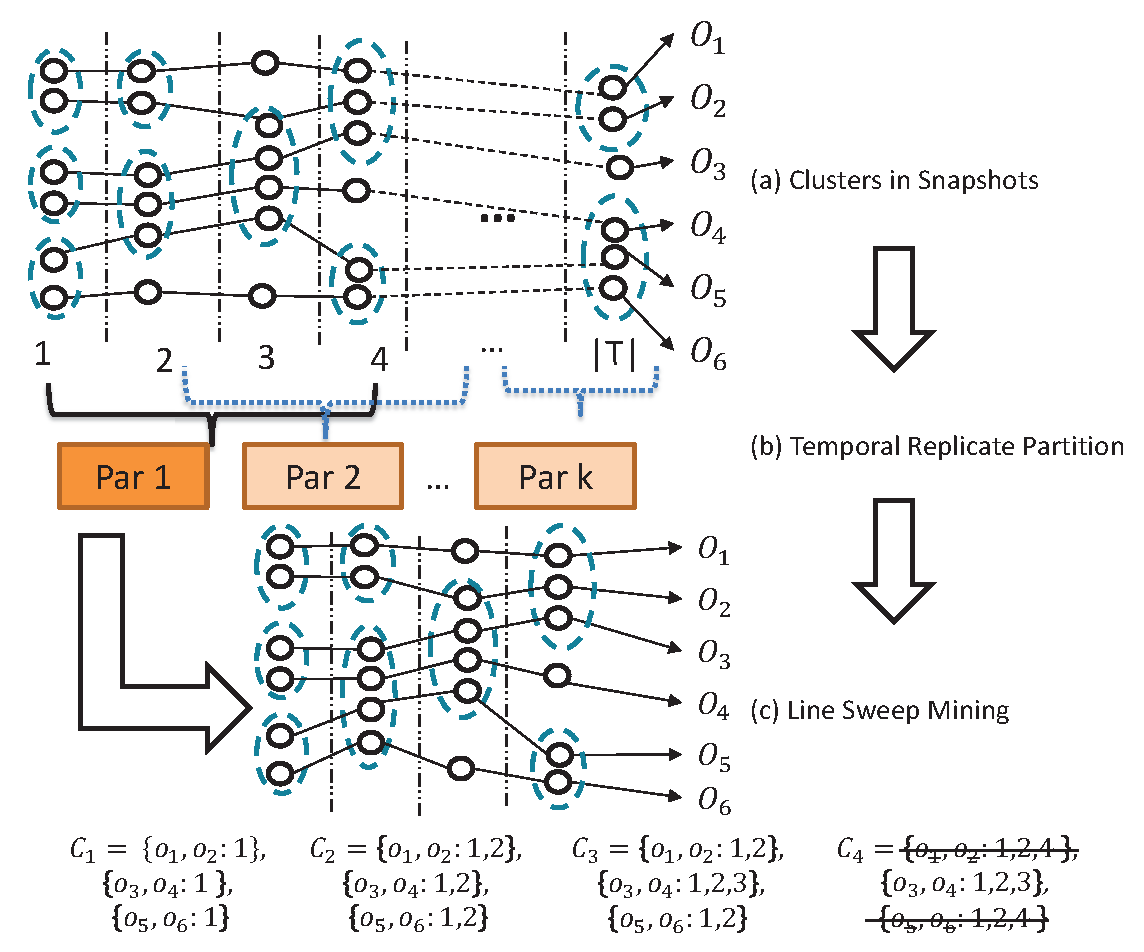
\includegraphics[width=0.5\textwidth]{trm_process.eps}
%\caption{Work flow of trajectory replication and mining}
%\label{fig:trm_process}
%\end{figure}

\subsection{Correctness of TRM}
We prove the correctness of TRM from two aspects. First,
the choice of $R = (\lceil \frac{K}{L} \rceil -1)*G+2K$ would 
not miss out any valid patterns. Second, no false patterns
are reported in any partitions. We formalize these two 
properties as \emph{completeness} and \emph{soundness} as follows:

\begin{definition}[Completeness and Soundness]
Let a partition method $\mathbb{P}$ partitions a trajectory database $Tr$ 
into segments, $Par_1,...,Par_m$. $\mathbb{P}$ is complete 
if for every valid pattern $P$ in $Tr$, $\exists Par_i$ s.t. $P$ is valid in $Par_i$. 
$\mathbb{P}$ is sound if for all patterns that are valid in any $Par_i$, they are also valid in $TR$.
\end{definition}

Apparently, in TRM, replicating the entire trajectories (i.e., $R=\mathbb{|T|}$)
meets the \emph{soundness} and \emph{completeness} requirements. However, it burdens the network shuffle and limits the parallelism. We carefully chose $R = (\lceil \frac{K}{L} \rceil -1)*G+2K$ and use
the following theorem to state the correctness:

\begin{theorem}[Correctness of Replication]
\label{thm:replication_partition}
Temporal replication partition is sound and complete.
\end{theorem}z
\begin{proof}
The soundness of partition can be observed from the fact 
that each partition represents a consecutive segments of trajectories. 
Therefore patterns in a partition can be directly mapped 
back to original trajectories. For completeness, with a
valid pattern $P$, let $T'$ be the subsequence of $P.T$ which conforms to $K,L,G$ 
with the smallest length. Note that there could be many qualified $T'$s. 
Let the $i^{th}$ local-consecutive segment of $T'$ be $l_i$ and 
let the $i^{th}$ gap of $T'$ be $g_i$. Then, the size of $T'$ can 
be written as $\Sigma_i (l_i + g_i)$.  Since $T'$ conforms to $K,L,G$, 
then $2K \geq \Sigma_i (l_i) \geq K$, $l_i \geq L$, $g_i \leq G$. 
It follows: $\Sigma_i(l_i+g_i) \leq (\lceil \frac{K}{L} \rceil -1) *G+2K$. 
If every partition is of at least such a size, then $T'$ must be
captured by at least one of the partition. Thus, the pattern $P$ would 
be valid in that partition. This proves the completeness.
\end{proof}

\begin{example}
We illustrate the work flow of  TRM method using Figure~\ref{fig:trm} (c)(d) with $M=2, K=2, L = 2, G=2$. 
In Figure~\ref{fig:trm} (c), snapshots are combined into partitions with sizes equal to 
$(\lceil \frac{K}{L} \rceil-1) *G+2K = 4$. Then a line sweep method is performed in (d) 
for partition $1$. Each $C_i$ refers to the candidate set during sweeping snapshot $i$. 
Initially, $C_1$ contains patterns whose object set is in snapshot $1$.
As line sweeps, at snapshot $4$, since the timestamps of $\{o_1,o_2\}$ and $\{o_5,o_6\}$ 
are both $\{1,2,4\}$ which violate the $G$ constraint, 
thus the two candidates are removed from $C_4$. After all snapshots are swept, 
$\{o_3,o_4\}$ is the qualified pattern and is outputted.
\end{example}

The TRM approach though achieves good parallelism, 
it requires to replicate the data multiple times. 
Specifically, each snapshots are replicate $(\lceil \frac{K}{L} \rceil -1) *G+2K$ times. 
In the cases of \emph{swarm}, \emph{group} and \emph{platoon}, $G$ is as large as $|T|$. 
Handling those cases is equivalent to replicate the entire snapshots to each partition, 
which surrenders the benefit of parallelism.



%IMPORTANT!!!
%In contrast, it is challenging to design the second job. 
%This is because valid patterns may spray across multiple snapshots 
%or contain different object sets, where inappropriate partitioning
%of snapshots may fail to discover certain valid patterns.
%Formally, a valid partition strategy 
%needs to meet the following requirements: (a) the resulted partitions need
%to preserve enough information so that real patterns can be discovered in the reduce phase. 
%(b) the resulted partitions need to ensure that
%the patterns discovered in the reduce phase are valid patterns so that
%no further verification is required. We formalize these two 
%properties as \emph{completeness} and \emph{soundness} as follows:
%
%\begin{definition}[Completeness and Soundness]
%Let a partition method $\mathbb{P}$ partitions original trajectories $Tr$ into multiple parts, $Par_1,...,Par_m$. $\mathbb{P}$ is complete if for every pattern $P$ that is valid in $Tr$, $\exists Par_i$ s.t. $P$ is valid in $Par_i$. $\mathbb{P}$ is sound if for all patterns that are valid in any $Par_i$, they are also valid in $TR$.
%\end{definition}
%The completeness ensures that no true patterns are missed out. 
%The soundness ensures that no false patterns are reported. 
%If a partition method is both sound and complete, then it can be used
%in the second MR job to facilitate GCMP mining.
%
%Apparently, replicating the entire trajectories to each 
%partition meets the \emph{soundness} and \emph{completeness} requirements. 
%However, it burdens the network shuffle and limits the parallelism. 
%Our objective is thus to design a complete and sound partition method that minimize the network shuffles.
%In the following sections, we describe a naive \emph{temporal-based} partition-and-mining method called \emph{Temporal Replication and Mining}(TRM) towards a parallel solution of GCMP mining. Then,
%we present a novel \emph{object-based} partition-and-mining method
%called \emph{Star Partition and Mining} (SPM) which resolves
%the deficiencies of TRM method.
